\chapter{緒論}\label{ch:intro}

\section{研究背景}\label{sec:background}

因子投資的研究長期累積了大量可用於選股的公司特徵，從規模與價值\parencite{famafrench1993}到獲利、品質等構面，使量化投資者得以將投資邏輯寫成明確的規則，進而回測、驗證並重複執行。然而，因子數量的膨脹也帶來所謂「因子動物園」（factor zoo）的問題：\textcite{fenggiglioxiu2020}即以「馴服因子動物園」為題，指出文獻中已有數百個因子被提出，而其中多數在既有因子之外並無額外的解釋力；\textcite{harveyliuzhu2016}則指出，當數百個因子被反覆檢定時，單憑運氣也會找到看似有效的因子，因此新因子必須通過比傳統更嚴格的顯著性標準，才能被視為可信。

近年來，運算資源與大型語言模型（Large Language Model, LLM）的發展，使策略與因子的生成成本進一步下降。LLM 驅動的因子挖礦框架能夠自動生成並反覆迭代大量候選因子~\parencite{tang2025alphaagent, wang2026factorminer}，即使不借助 LLM，宣告式的回測引擎也能以規則窮舉的方式批量產出候選策略。生成能力不再是稀缺資源，策略池的規模因而快速擴張。

然而，策略數量的擴張並不等於資訊的擴張。有研究指出，因子庫愈大，尋找新訊號愈困難，因為大量因子之間高度冗餘~\parencite{wang2026factorminer}；亦有研究把因子的同質化與 alpha 衰減視為因子挖礦必須對抗的問題~\parencite{tang2025alphaagent}。另一方面，已被發現的報酬可預測性在樣本外與發表之後會出現衰減~\parencite{mcleanpontiff2016}，意味著任何一組在歷史上表現良好的策略，都不能被假設會持續有效。

策略所處的市場本身也在變動。以美國為例，標普 500 指數前十大成分股的市值占比在 2024 年已接近百年來的最高水準，約為 36\%~\parencite{goldman2024concentration}。當指數的報酬由少數權值股主導時，等權或接近等權、強調分散的量化策略組合，即使選股規則本身沒有失效，其表現也可能長時間偏離市值加權的大盤。策略池因此不是建好之後就能放著不管，而需要被持續監控與修正。

此外，在機構實務上，投資決策還必須能被解釋、稽核與治理。LLM 與 AI 代理人在金融領域的應用正快速擴張~\parencite{aldridge2026agentic}，為解釋與輔助決策提供了新的工具，卻也帶來新的風險：LLM 的輸出可能來自對訓練資料的記憶，而非真正的推理~\parencite{jeonlee2026blindfolded}，在以歷史資料進行的回測中尤其難以排除。

承接前述，因子與策略的生成成本持續下降，使策略池的規模不斷擴張；但規模擴張同時帶來冗餘、衰減與市場結構變動的挑戰，而機構又要求決策流程能被解釋與稽核。如何在這樣的環境下，從大量機器生成的策略中找出真正獨立的分散來源、持續監控並於必要時修正，並以可驗證的方式輔助解釋決策，正是本研究的出發點。

\section{研究動機}\label{sec:motivation}

基於上述研究背景，本研究的動機主要來自四個層面。

首先，在策略池的規模與分散方面，背景指出策略數量龐大並不等於資訊相互獨立，而在大量策略被反覆檢定的情況下，「從中挑出表現好的」本身就帶有資料窺探的疑慮。既有針對 LLM 因子挖礦的研究多著眼於\textbf{生成階段}，以正規化或記憶機制降低冗餘~\parencite{tang2025alphaagent, wang2026factorminer}；然而，對於一個已經生成的大型策略池，它真正獨立的程度有多高、能否從中挑選出具代表性的子集，以及這樣的挑選相較於「全部買進」與隨機抽樣是否真有價值，仍需要一套生成之後的診斷與驗證方法。此外，生成的策略並非全數可用，須先標記其資料品質是否合格、全期間報酬是否優於基準，才能進入後續分析（第\ref{sec:research}節）。

其次，在持續有效性方面，策略的優勢可能衰減，市場結構也會變動，這使得一次性的挑選不足以支撐實戰。我們需要知道：在樣本外持續監控、偵測投資組合與歷史假設之間的偏離，並於必要時加以修正，是否真的比「不做任何調整」更好，而不是假設調整機制天然有益。

再者，在可解釋性與治理方面，真實的基金機構要求決策留下稽核紀錄並能向人說明；以 LLM 輔助解釋雖然可行，但須處理幻覺與訓練資料污染的風險，且其可信度必須被實際檢驗，而非預設成立。

最後，在市場適用性方面，台灣與美國在市場規模、指數編製與集中度結構上並不相同。若一套方法論只在單一市場成立，其價值有限；因此，需要在台股與美股兩個市場各自獨立驗證，以檢驗方法論是否僅為單一市場的特例。

換言之，無論候選策略是由 FCV 這類宣告式引擎、LLM 因子挖礦，還是梯度提升樹（gradient boosting）等機器學習工具所產生，產出本身都不再是瓶頸；本研究關切的，是這些策略生成\textbf{之後}如何被治理——是否分散、能否被持續監控與修正、決策能否被解釋與稽核。下一節將此一關切拆解為一個主軸與三個可檢驗的子問題。

\section{問題意識}\label{sec:questions}

為回應上述動機，本研究以模擬一個量化基金公司（Fund House）的完整投資流程作為實驗情境：首先以宣告式多因子回測引擎（Factor–Condition–Valuation，以下簡稱 FCV）系統性地產出大量候選選股策略；接著由研究部（以基金公司的組織作比喻，負責分析整個策略池的分析層）透過階層式分群分析這批策略，找出其中真正獨立、互補的分散來源，並據此挑選代表策略、組成精選組合；最後在實戰應用層（負責持續運作投資組合的決策層）持續監控組合現況，於必要時動態調整，並由 LLM 代理人輔助解釋每一項決策。整條流程分別在台灣與美國兩個股票市場獨立驗證，其全貌如圖\ref{fig:overview}所示。

\begin{figure}[htbp]
  \centering
  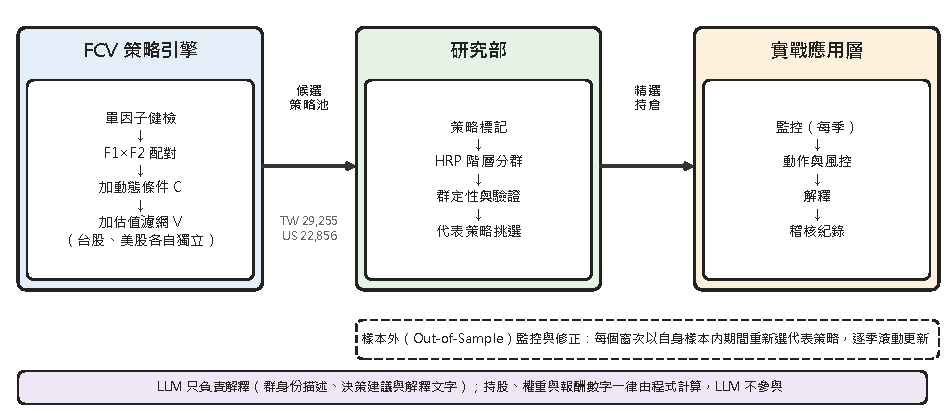
\includegraphics[width=\textwidth]{fig_overview.pdf}
  \caption{投資流程總覽：FCV 策略引擎、研究部與實戰應用層}\label{fig:overview}
\end{figure}

FCV 採用宣告式的設計：使用者不逐一撰寫策略，而是從三個維度宣告策略的規格——F（體質因子，決定選擇什麼樣的公司）、C（動態條件，決定進場的時間點是否恰當）與 V（估值濾網，決定價格是否過高）——由引擎窮舉各維度的組合並完成回測，因而能以系統化、可重複的方式產出上萬檔候選策略。引擎的設計細節於第\ref{sec:fcv}節說明；就本研究而言，FCV 只是能大量產生策略的來源之一，其產出才是後續兩層所要處理的對象。

此一投資流程可視為由三個環節逐層疊加而成：策略擴張（FCV）、精選（研究部）與調整（實戰應用層）。本研究以兩種最簡單的做法作為對照——「全部買進」（將候選池中所有可用策略等權持有，記為 B\_all）與「不做任何調整」——並據此提出本研究的\textbf{主軸}：

\begin{quote}
投資流程中逐層增加的環節——策略擴張、精選、調整——是否各自在樣本外（Out-of-Sample）帶來可驗證的額外價值？
\end{quote}

此處的「價值」從報酬、風險、分散與互補四個面向衡量；加上「樣本外」這個限定，是為了讓精選與調整兩個環節落在同一個驗證邏輯之下，而非各自採用不同強度的證據標準。主軸進一步拆解為三個子問題（Sub-Question，以下簡稱 SQ）與一項外部效度檢查：

\begin{description}
  \item[SQ1（擴張）] 大量策略是否帶來真正的獨立性與互補性（亦即所謂的「免費午餐」）？這種互補性存在於台股—台股、美股—美股，還是台股—美股的配對之中？
  \item[SQ2（精選）] 精選是否優於全部買進與隨機抽樣？
  \item[SQ3（調整）] 動態調整是否優於不動作？
  \item[外部效度] 以上結論在台股與美股是否方向一致？
\end{description}

其中，SQ1 與 SQ2 對應第三章第\ref{sec:research}節的研究部方法論，SQ3 對應第\ref{sec:app}節的監控決策系統設計；第\ref{sec:fcv}節僅介紹 FCV 工具，不直接回答任何一個子問題。第四章依序以實證回答三個子問題，再以台美兩個市場的比較檢驗結論的普適性；最後，第五章在四項答案齊備之後，才回到最上方的主軸作總結。

為避免對研究範圍產生誤解，須先界定三項邊界。第一，三個子問題皆為「是否、差異多少」的事實問題，而非「如何做」的工程問題。第二，LLM 解釋的可信度是系統元件的驗證，而非研究問題本身：本研究並非追問「LLM 本質上是否可信」這類開放問題，而是檢驗本研究所設計的抗幻覺機制是否達到預先設定的驗證標準（第\ref{sec:explain}節、第\ref{sec:forward}節與第\ref{sec:llm-validation}節）。第三，SQ3 所依據的實證證據，主要來自台股一段特定期間（2024 至 2025 年）的連續事件，美股在同一期間僅有極為有限的觸發紀錄，因此屬於探索性案例，不宜作為長期結論。明確界定這些邊界，是方法論嚴謹的一部分，而非對弱點的迴避。

\section{研究目的與貢獻}\label{sec:contribution}

針對上述動機、主軸與子問題，本研究的目的與貢獻有以下四點。

\begin{enumerate}
  \item \textbf{建立並驗證可重複使用、可擴展至不同市場的宣告式多因子回測引擎（FCV）。}它是達成後續三項目的的工具，如前所述，也只是能大量產生策略的來源之一，因此本論文對其篇幅著墨不多。
  \item \textbf{量化策略池的真實分散程度，並提出精選為何有效的解釋。}本研究以階層式分群（Hierarchical Risk Parity 之分群步驟，\textcite{lopezdeprado2016hrp}）與有效獨立賭注數（Effective Number of Bets, ENB；\textcite{meucci2009}）量化策略池的分散程度，回答 SQ1；並進一步提出精選規則為何能創造價值的具體機制，回答 SQ2，而不僅止於揭露「表面分散是假象」。
  \item \textbf{建構具備監控、調整、風控、解釋與治理的實戰應用系統，並使其流程在樣本外成立。}該系統包含集中度與覆蓋率監控、條件式市值傾斜調整、持股與回測偏離風控、七段式解釋與投資政策聲明（IPS）／董事會備忘錄式的治理設計（回答 SQ3），並以前瞻驗證在排除 LLM 訓練資料污染的條件下，檢驗解釋機制的可信度。這套系統能持續以樣本外監控隔離近期的偏離並執行修正，這是它與「單純能批量產生策略」的工具之間最根本的差異，也是本研究方法論貢獻的核心。
  \item \textbf{在台股與美股兩個市場各自獨立驗證整套方法論。}此舉用以支持方法論並非單一市場特例的論點，並誠實呈現兩個市場結果的差異與證據強度的不對等。
\end{enumerate}

第三點須特別釐清其範圍：此處主張的是「\textbf{流程本身在樣本外成立}」，而非「樣本外績效必然勝過大盤」。後者在本研究目前的證據下仍相當薄弱——SQ3 的證據僅限於一段特定期間，且在台股含 LLM 代理人決策的完整模擬中，同一設定下僅因代理人所見輸入內容的差異，結果就相差達數十個百分點，無法據以判定方向。前者則來自系統設計本身所具備的四項流程特徵，與具體的績效數字無關：(1) 每個驗證窗口都以自身的樣本內期間重新挑選代表策略，不借用該窗口之後的資訊（但候選池本身是以全期間表現篩出，此一偏誤於第\ref{sec:limitations}節說明）；(2) 調整動作設有一季的決策延遲；(3) 逐季滾動更新；(4) 前瞻驗證刻意採用 LLM 訓練截止日之後的真實時點，以排除模型背誦答案的可能。這四項特徵皆可獨立檢驗，不依賴「這一次剛好贏過大盤」這個脆弱的結果。

最後，本研究在過程中誠實記錄了數個被後續證據推翻或降級的中間結論，並於第\ref{sec:conclusions}節與第\ref{sec:limitations}節說明其意義。

\section{論文結構}\label{sec:thesis-structure}

本論文共分五章。第一章為緒論，說明研究背景、動機、問題意識與研究目的。第二章回顧相關文獻，涵蓋因子投資理論、多因子模型與方法論（包含階層風險平價與有效獨立賭注數）、監控決策系統與 LLM 代理人的相關文獻、績效與風險指標，並在最後一節定位本研究相對於既有文獻的位置與缺口。

第三章說明系統設計與實作：第\ref{sec:fcv}節簡述 FCV 引擎；第\ref{sec:research}節建立研究部分析策略池所用的方法論，對應 SQ1 與 SQ2；第\ref{sec:app}節說明實戰應用層的監控、動作、風控、解釋、前瞻驗證與治理設計，對應 SQ3，並以對照表彙整每個設計項目在第四章的驗證位置。

第四章呈現實證結果：第\ref{sec:pool}節說明台美股的候選池建構；第\ref{sec:structure}節回答 SQ1 與 SQ2；第\ref{sec:tw}節與第\ref{sec:us}節分別呈現台股與美股專屬的機制驗證，涵蓋 SQ3；第\ref{sec:cross}節依事先設定的判準比較兩個市場，檢驗外部效度；第\ref{sec:llm-validation}節完成 LLM 解釋代理人這個系統元件的前瞻驗證。第五章回扣第一章提出的主軸與子問題，總結研究結論、限制與未來研究方向。

下一章首先回顧支撐本研究方法論與系統設計的相關文獻。
